\chapter{Introduction}
\label{chap:intro}

\section{Motivation}
\label{chap:motivation}

These days witness the development of information extraction methods, which are fruitfully exploited for automatic construction of KGs, that is, large collection of relational facts with the RDF~\cite{ref38} format $\langle subject \rangle \langle predicate \rangle \langle object \rangle$. These are triples reflecting facts about the real world which can be converted to facts over unary and binary relations in predicate calculus. Indeed, the unary, binary relations are corresponding to the RDF fact with $\langle type \rangle$ and other predicates, respectively. For example, $\langle Brad \rangle \langle livesIn \rangle \langle Berlin \rangle$ can be rewritten as $livesIn(Brad, Berlin)$ while $\langle Mat \rangle \langle type \rangle \langle artist \rangle$ can be converted to $artist(Mat)$. Examples of KGs include the YAGO~\cite{ref28}, FreeBase~\footnote{\url{https://developers.google.com/freebase/}}, etc (see Chapter~\ref{chap:relwork} for details).

KGs are normally incomplete due to automatic construction. Hence, they should be processed under the Open World Assumption (OWA). The \textit{knowledge completion problem} (also known as \textit{link prediction}) plays an important role in improving the quality of KGs. To achieve this, rule learning approaches~\cite{ref39, ref10} are used to create rules which can infer new potentially missing facts. However, the existing methods only pay attention to positive rules, which do not take exceptions or negated atoms into consideration and may infer wrong facts. To be specific, a rule:

\begin{center}
$r1: livesIn(Y,Z) \leftarrow isMarriedTo(X,Y), livesIn(X,Z)$
\end{center}

can be discovered from the graph in the Figure~\ref{fig1.1} and exploited to predict new facts $livesIn(Alice, Berlin), livesIn(Dave, Chicago)$ and $livesIn(Lucy, Amsterdam)$. It can be seen that the first two triples are incorrectly predicted because $Alice$ and $Dave$ are researchers and the rule $r1$ cannot be applied to them. Thus, mining exceptions should be taken into account to improve the rule quality and producing precise relations.

\begin{figure}[t]
\centering
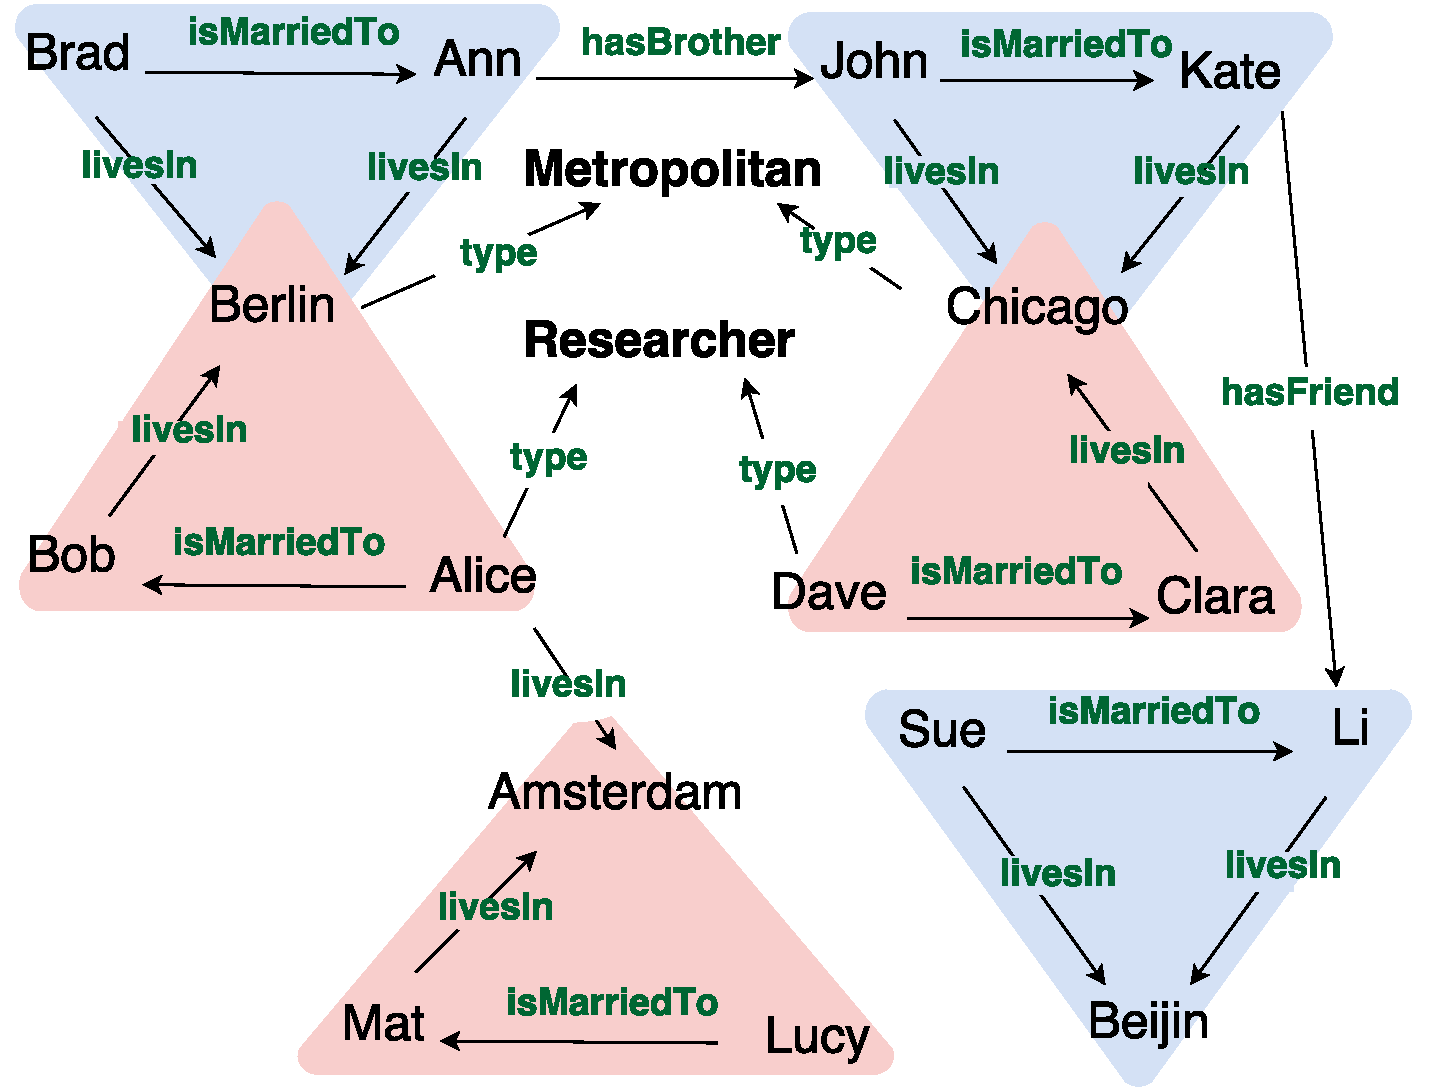
\includegraphics[width=0.75\textwidth]{figures/kg_advanced_col}
\caption{A Visualization of a Knowledge Graph}
\label{fig1.1}
\end{figure}

\section{Challenges}

Exception mining problem has been addressed in \textit{nonmonotonic learning programs}~\cite{ref11, ref40, ref41, ref32, ref42}. Nonetheless, some state-of-the-art nonmonotonic ILP algorithms cannot be applied directly to our problem. Firstly, the \textit{target relations} are hard to clearly indicated because we do not know which components in the graph need to be extended. A naive solution to this issue is mining all possible rules from the available predicates at hand. However, this way is not promising due to the big volume of facts in the original KGs. Secondly, \textit{negative facts} are difficult to collect because i) we sometimes cannot differentiate between wrong and unseen triples and ii) there are a lot of facts in KGs. Thus, a simple approach to overcome this is exploring rules from solely positive facts. Finally,  the \textit{language bias} is not easy to define since the schema of original data is not given. To tackle this, we assume the specific form of the positive rules in Chapter~\ref{chap:system}.

To overcome the above obstacles, exploratory data mining solution is a suitable choice. The authors in~\cite{ref12} proposes association rule mining methods to explore Horn positive rules, and then revise them by inserting exceptions or negated atoms in their body to improve predictive quality. Nonetheless, it only works on flattened presentation of KG, that is, a collection of unary projected facts.

\section{Contributions}

This thesis is an extension from publication~\cite{ref12} where we want to mine rules with exceptions in the nature form of KGs. To be specific, the knowledge completion problem is transformed to \textit{theory revision} one, in which \textit{nonmonotonic rules} are explored given an original KG and Horn rules. The positive rules can be found by using off-the-shell tools in the literature. Besides, we expect that the quality of revised rules is better than that of original positive ones with respect to a specific measure.

There are four steps in our system. Firstly, for each positive rule, we try to find normal and abnormal sets, that is, set of instances that follow or do not follow a given rule, respectively. Secondly, we mine exception witness sets, that is, set of unary or binary relations that can eliminate abnormal instances. To be specific, \textit{Researcher} is an example for this in Figure~\ref{fig1.1}. Thirdly, we add exceptions to the Horn rules and define a measure to assess rule quality. Besides, the interaction between revised rules can be taken into consideration by a novel concept of \textit{partial materialization}. Finally, exceptions are ranked based on the measure and the revised rules are expected to have both descriptive and predictive qualities.

The contributions of this thesis are three-fold:

- We introduce a theory revision framework to capture negated atoms, this is a rule-based method for KG completion problem.

- We propose a method for finding exception candidates, assessing their quality and ranking them based on choosen measure. Especially with the novel concept of \textit{partial materialization}, the cross-talk between the revised rules are concerned.

- We conduct experiments with YAGO3 and IMDB datasets to test the above-mentioned methodology and partial materialization concept.

\section{Structure}

The outline of this thesis is as follows. Chapter~\ref{chap:relwork} mentions related work and literature review. Chapter~\ref{chap:back} provides background and preliminaries for nonmonotonic and association relational learning. Chapter~\ref{chap:frame} proposes the problem of theory revision and our methodology. Chapter~\ref{chap:system} describes system overview, implementation details and optimization. Chapter~\ref{chap:eval} indicates the result of the experiment for YAGO and IMDB KGs and Chapter~\ref{chap:conclusion} is a conclusion for the thesis.